\documentclass{beamer}
\usetheme{Madrid}
\usepackage{amsmath}
\usepackage{listings} % For including code
\usepackage{booktabs} % For cleaner tables

% Professional code styling
\lstset{
    language=Python,
    basicstyle=\ttfamily\small,
    keywordstyle=\color{blue},
    commentstyle=\color{gray},
    breaklines=true,
    frame=single
}

\title{Discrete Signal Processing}
\author{Arsh Dhoke \\ Roll No. EE25BTECH11010}
\date{}

\begin{document}

\frame{\titlepage}

\begin{frame}{The Problem Statement}
    \textbf{Question 1.2.10 (GATE CS 2007):}\\
    Consider the series $x_{n+1} = \frac{x_n}{2} + \frac{9}{8x_n}$, $x_0 = 0.5$ obtained from the Newton-Raphson method. The series converges to:
    \vspace{0.5cm}
    \begin{enumerate}[a)]
        \item 1.5
        \item $\sqrt{2}$
        \item 1.6
        \item 1.4
    \end{enumerate}
\end{frame}

\begin{frame}{The Theorem: Limit of a Convergent Sequence}
    \textbf{Theorem:}\\
    If a recursive sequence given by a continuous function $x_{n+1} = f(x_n)$ converges to a limit $L$, then $L$ is a fixed point of $f$. That is, $L = f(L)$.
    
    \vspace{0.3cm}
    \textbf{Proof:}\\
    Taking the limit of both sides of our recurrence relation:
    \begin{align*}
        \lim_{n \to \infty} x_{n+1} &= \lim_{n \to \infty} f(x_n)
    \end{align*}
    Because $f$ is a continuous function, we can pull the limit inside:
    \begin{align*}
        L &= f\left(\lim_{n \to \infty} x_n\right) \implies L = f(L) 
    \end{align*}
\end{frame}

\begin{frame}{Solution}
    Let the series converge to $L$. Substituting $L$ into the recurrence relation:
    \begin{align*}
        L &= \frac{L}{2} + \frac{9}{8L} \implies \frac{L}{2} = \frac{9}{8L} \\
        4L^2 &= 9 \implies L = \pm 1.5
    \end{align*}
    Since $x_0 = 0.5 > 0$, and the sequence terms remain positive, it converges to:
    \begin{align*}
        L &= 1.5
    \end{align*}
    \textbf{Correct Answer:} a) 1.5
\end{frame}

\begin{frame}{Simulation Output}
    \begin{center}
        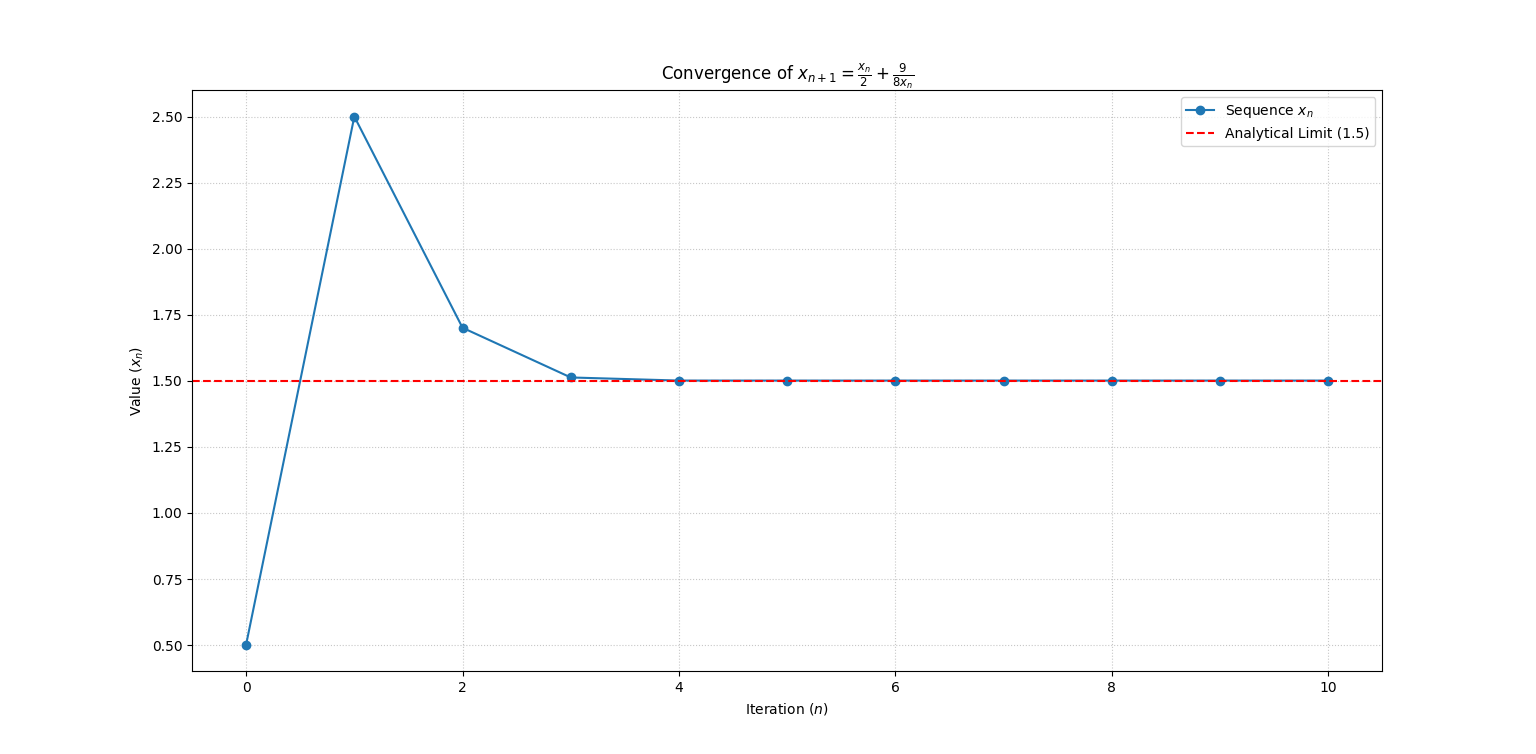
\includegraphics[height=6cm]{Figure_2.png} 
    \end{center}
\end{frame}
\begin{frame}[fragile]{Numerical Simulation (Python)}
    \vspace{0.3cm}
    \textbf{Simulation Output:}
    \begin{center}
    \begin{tabular}{ccccccc}
    \toprule
    $n$ & 0 & 1 & 2 & 3 & 4 & 5 \\ \midrule
    $x_n$ & 0.500 & 2.500 & 1.700 & 1.514 & 1.500 & 1.500 \\
    \bottomrule
    \end{tabular}
    \end{center}
    The sequence exhibits \textbf{quadratic convergence}, hitting 1.5 in just 4 iterations.
\begin{lstlisting}
import matplotlib.pyplot as plt

def simulate_sequence(x0, iterations):
    # Initialize list with the starting value
    x_values = [x0]
    
    print(f"{'Iteration':<10} | {'Value (x_n)':<15}")
    print("-" * 30)
    print(f"{0:<10} | {x0:<15.6f}")
\end{lstlisting}
\end{frame}
\begin{frame}[fragile]{Numerical Simulation (Python)}
\begin{lstlisting}

    for n in range(1, iterations + 1):
        # The recurrence relation: x_{n+1} = x_n/2 + 9/(8*x_n)
        current_x = x_values[-1]
        next_x = (current_x / 2) + (9 / (8 * current_x))
        x_values.append(next_x)
        
        print(f"{n:<10} | {next_x:<15.6f}")
        
    return x_values

# Parameters from your problem
x_initial = 0.5
num_iterations = 10
\end{lstlisting}
\end{frame}

\begin{frame}[fragile]{Numerical Simulation (Python)}
\begin{lstlisting}
# Run simulation
results = simulate_sequence(x_initial, num_iterations)

# Plotting the convergence
plt.figure(figsize=(10, 6))
plt.plot(range(len(results)), results, 'o-', label='Sequence $x_n$')
plt.axhline(y=1.5, color='r', linestyle='--', label='Analytical Limit (1.5)')
plt.title('Convergence of $x_{n+1} = \\frac{x_n}{2} + \\frac{9}{8x_n}$')
plt.xlabel('Iteration ($n$)')
plt.ylabel('Value ($x_n$)')
plt.grid(True, linestyle=':', alpha=0.7)
plt.legend()
plt.show()
\end{lstlisting}
\end{frame}

\end{document}